\documentclass[french]{article}
\usepackage{geometry}
\geometry{a4paper}
\usepackage{graphicx}
\usepackage{amssymb}
\usepackage{amsmath}
\usepackage{amsthm}
\usepackage{empheq}
\usepackage{mdframed}
\usepackage{booktabs}
\usepackage{graphicx}
\usepackage{color}
\usepackage{psfrag}
\usepackage{pgfplots}
\usepackage{bm}
\usepackage[utf8]{inputenc}
\usepackage[T1]{fontenc}
\usepackage{babel}
\usepackage{indentfirst}
\usepackage{float}

\definecolor{ocre}{RGB}{243,102,25}
\definecolor{mygray}{RGB}{243,243,244}

\newcommand\orangebox[1]{\fcolorbox{ocre}{mygray}{\hspace{1em}#1\hspace{1em}}}

\newtheoremstyle{mytheoremstyle}
    {3pt}
    {3pt}
    {\normalfont}
    {0cm}
    {\rmfamily\bfseries}
    {.}
    {1em}
    {{\color{ocre}\thmname{#1}~\thmnumber{#2}}\thmnote{\,--\,#3}}
\newtheoremstyle{myproblemstyle}
    {3pt}
    {3pt}
    {\normalfont}
    {0cm}
    {\rmfamily\bfseries}
    {.}
    {1em}
    {{\color{black}\thmname{#1}~\thmnumber{#2}}\thmnote{\,--\,#3}}
\theoremstyle{mytheoremstyle}
\newmdtheoremenv[
    backgroundcolor=mygray,
    linecolor=ocre,
    leftmargin=0pt,
    innerleftmargin=20pt,
    innerrightmargin=20pt,
]{theorem}{Theorem}[section]
\theoremstyle{mytheoremstyle}
\newmdtheoremenv[
    backgroundcolor=mygray,
    linecolor=ocre,
    leftmargin=0pt,
    innerleftmargin=20pt,
    innerrightmargin=20pt,
]{definition}{Definition}[section]
\theoremstyle{myproblemstyle}
\newmdtheoremenv[
    linecolor=black,
    leftmargin=0pt,
    innerleftmargin=10pt,
    innerrightmargin=10pt,
]{problem}{Problem}[section]

\usepgfplotslibrary{colorbrewer}
\pgfplotsset{width=8cm,compat=1.9}

\title{Approches Deep Learning à la détection d'anomalies dans un système à temps réel}
\author{Mohamed-Amine ROMDHANE, Adam FEOR}
\date{}

\begin{document}
    \maketitle

    \tableofcontents
    \clearpage

    \section{Introduction}
    Dans le cadre d'un besoin d'une startup spécialisée dans des services d'optimisation de consommation d'eau dans le milieu agricole, on veut pouvoir mettre en place un modèle de détection d'anomalies matérielles via les méthodes d'apprentissage automatique et de l'intelligence artificielle. Dans cette optique, cette entreprise a installé des senseurs sur des pompes à eaux qui en indiquant la pression à l'intérieur, permettent d'indiquer l'état d'irrigation. Celle-ci est déclenchée automatiquement à l'aide de capteurs d'humidité du sol.     
    \section{Problématique \& Hypothèses}
    Les senseurs de pression d'eau d'une pompe ne sont pas parfaits, et ils peuvent envoyer des valeurs légèrement différentes entre deux lectures. De plus, certains facteurs comme la chaleur ou l'humidité qui varient naturellement font en sorte que les courbes de ces senseurs ont toujours un bruit de basse amplitude. Il peut aussi arriver qu'une bulle d'air ou un petit objet passe temporairement par la pompe et devienne une "dent" sur le graphe de suivi de pression d'eau, c'est à dire une forte perturbation d'amplitude en un court moment.
    \newline
    \indent Le fonctionnement normal d'une pompe ressemble donc à une période calme perturbée uniquement par un bruit global, puis lorsque le capteur détecte que l'irrigation est nécessaire la courbe grimpe jusqu'à son maximum, et y reste jusqu'à ce que le capteur détecte que la terre est suffisamment irriguée. S'ensuit une chute brusque de la pression puis un retour au calme jusqu'au prochain cycle.
    \newline
    \indent Dans le cadre de cet étude, on a deux problèmes. Le premier est celui de la disponibilité des données. Le contact limité avec l'entreprise en ai une raison. Le second problème c'est que le modèle réel a beaucoup trop de variables, les senseurs dépendent les uns des autres et les bruits ainsi que les anomalies ont plusieurs sources et facteurs. 
    \newline
    \indent Le but de ce projet est au final de développer des approches d'apprentissage profond. Avec le peu de données qu'on a, la solution était de faire nos propres données qui s'approchent au mieux de ce qu'on nous a communiqué.
    \section{Les données}
    Faute de manque de données, nous nous sommes fixés la  création d'un outil permettant de générer des courbes d'états ressemblant à celles utilisés par l'entreprise. Cet outil devrait être modulaire pour permettre de simuler toutes les situations auxquelles l'entreprise est confrontée, incluant les anomalies. Il faut donc prévoir des paramètres permettant de varier le temps entre les cycles de pression, le nombre d'anomalies, leur type, le bruit, la fonction de transition entre états, etc...
        \subsection{Simulation des données}
        Le simulateur \textit{simulator.py} simule un système à temps réel. Ce dernier regroupe plusieurs variables dont:
        \begin{itemize}
            \item \textbf{realtime\_tick} l'écroulement temporel en millisecondes avant l'enregistrement d'un échantillon. Cette variable s'incrémente par \textit{dt\_per\_sample} après chaque échantillon.
            \item \textbf{dt\_per\_sample} c'est le temps en secondes entre chaque étape de simulation (temps entre deux échantillons).
            \item \textbf{transition\_type} est la fonction de transition entre états (exemple: East-In-Out Quad, Ease-In-Out Sine, Linear...).
            \item \textbf{noise} est la fonction de bruit global (exemple: "gaussian" pour un bruit gaussien).
            \item \textbf{states} est la liste d'états. Chaque état a une durée, une amplitude, et la liste (vide ou pas) des anomalies (appelées impulsions dans le contexte de simulation). Une anomalie a sa propre durée, le temps de son début ainsi que son amplitude.
        \end{itemize}
        \subsection{Génération des données}
    \section{Deep Learning avec TensorFlow}
        \subsection{Approche naïve avec CNN}
        La première idée qu'on a eu était d'utiliser le réseau neuronal convolutif de TensorFlow (convolutional neural networks, abbrv: cnn) pour l'entraîner à reconnaître les images provenant d'un système stable ainsi qu'un système à forte perturbations admettant plusieurs anomalies. Vu que précédemment on a déjà généré 1000 images pour chacune de nos classes \textbf{stable} et \textbf{malfunction}, on les a alors importées pour être pré-traitées avant de les brancher au réseau. Dans le prétraitement, on redimensionne la taille de l'image (originalement 640x480) à 250x250 et on redéfini la gamme de couleur de l'image comme étant \textit{greyscale}. On défini le nombre d'\textit{epochs} comme étant égale à 100 et le nombre de \textit{batchs} de données à être traité simultanément dans le réseau de neurones est égale à 8. Notre modèle TensorFlow a le pipeline décrit ci-dessous:
        \begin{center}
            Une \textbf{couche de convolution} à 2 dimensions avec \textbf{16} filtres, un noyau de taille \textbf{11x11} et la fonction de correction \textbf{RELu}. \\
            $
            \downarrow
            $\\
            Une \textbf{couche de pooling} où on prend que le \textbf{maximum} à l'issue des résultats précédents. \\
            $
            \downarrow
            $\\
            Une \textbf{couche de convolution} à 2 dimensions avec \textbf{32} filtres, un noyau de taille \textbf{11x11} et la fonction de correction \textbf{RELu}. \\
            $
            \downarrow
            $\\
            Une \textbf{couche de pooling} où on prend que le \textbf{maximum} à l'issue des résultats précédents. \\
            $
            \downarrow
            $\\
            Une \textbf{couche de convolution} à 2 dimensions avec \textbf{64} filtres, un noyau de taille \textbf{11x11} et la fonction de correction \textbf{RELu}.\\
            $
            \downarrow
            $\\
            Une \textbf{couche entièrement connectée} avec \textbf{512} neurones et une fonction d'activation \textbf{RELu}.\\
            $
            \downarrow
            $\\
            Une seul neurone avec la fonction d'activation \textbf{Sigmoïd}.
        \end{center}
        Avec 
        \[
        RELu(x) = \begin{cases}
            x,& \text{si } x \ge 0\\
            0,& \text{sinon}
        \end{cases}
        \]
        et
        \[
        Sigmoid(x) = \dfrac{1}{1+e^{-x}}
        \]
        \begin{figure}[H]
            \centering
            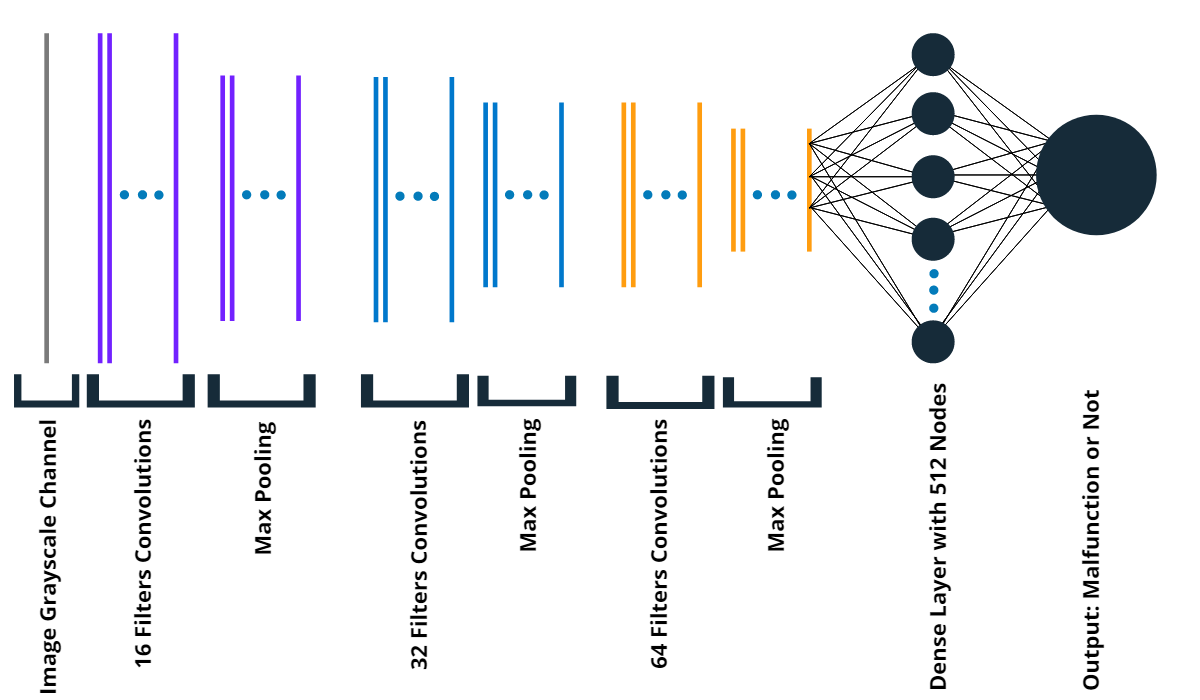
\includegraphics[width=\textwidth]{images/cnn.png}
            \caption{Le modèle CNN de classification d'anomalies}
            \label{}
        \end{figure}
        Notre modèle est compilé avec 2 ensembles d'images distincts. Un ensemble d'images d'entraînement et un ensemble de validation. En total, on a 2200 images pour l'entraînement et 2200 images pour la validation.
        \newline
        \begin{itemize}
            \item L'ensemble d'entraînement comporte 1100 images étiquetées \textbf{stable} ainsi que 1100 images étiquetées \textbf{malfunction}.
            \item L'ensemble de validation comporte le même nombre d'images pour chacune des deux classes mais des instances différentes de ceux dans l'ensemble l'entraînement.
        \end{itemize}
        \subsection{Génération des features avec TSFresh}
        \subsection{Détection d'anomalies en tant qu'objets}
    \section{Analyses et Interprétations}
    \section{Conclusion}
\end{document}